%!TEX root = ../paper.tex
\section{Video Classification in Caffe}
\label{sec:classification}

For building our artificial neural network we used the Caffe\footnote{\url{http://caffe.berkeleyvision.org/}} framework.
Caffe is a deep learning framework offering several implementations of common layers.
The source code for Caffe is hosted on GitHub available to be adapted and extended for special use cases.
We worked with the Caffe branch of Jeff Donahue\footnote{\url{https://github.com/BVLC/caffe/pull/2033}}, which offers an implementation for long-short-term memory (LSTM) networks.

Wu at al \cite{wu2015modeling} proposed a hybrid deep learning for video classification resulting in a complex artificial neural network architecture.
It comprises of three components: the \emph{spatial}, \emph{flow} and \emph{fusion} nets respectively.

The \emph{spatial} part is processing the single frames of a video in order to recognize objects and structures in frames.
The \emph{flow} part memorizes motion of actions by learning the optical flow images.
Both parts consist of a convolutional neural network (CNN) followed by a long-short-term memory (LSTM) recurrent neural network (RNN).
To merge the predictions of both parts, \emph{spatial} and \emph{flow}, a third part is introduced.
This part, called \emph{fusion}, takes the output of both CNNs and merges their predictions.
Hence the final overall prediction is a combination of the three results.

% COMMENT: Wir haben das nur mäßig getestet und damals gab es glaube auch noch die ein oder andere Unstimmigkeit in den Daten, aber damals haben wir ein eher mäßige Verbesserung von 1% oder so bekommen, während das entsprechende Paper deutlich mehr versprochen hatte, oder so...
Our initial test indicated that the use of LSTMs did not improve our prediction results.
Therefore we eliminated the LSTM parts for our network structure, leaving us more in line with two-stream approach of Simonyan et al\cite{simonyan2014two}, as shown in Figure~\ref{fig:architecture}.
The simplified approach retains a separate CNN's for spatial and flow as well as the fusion network.

\begin{figure}[!htb]
	\centering
	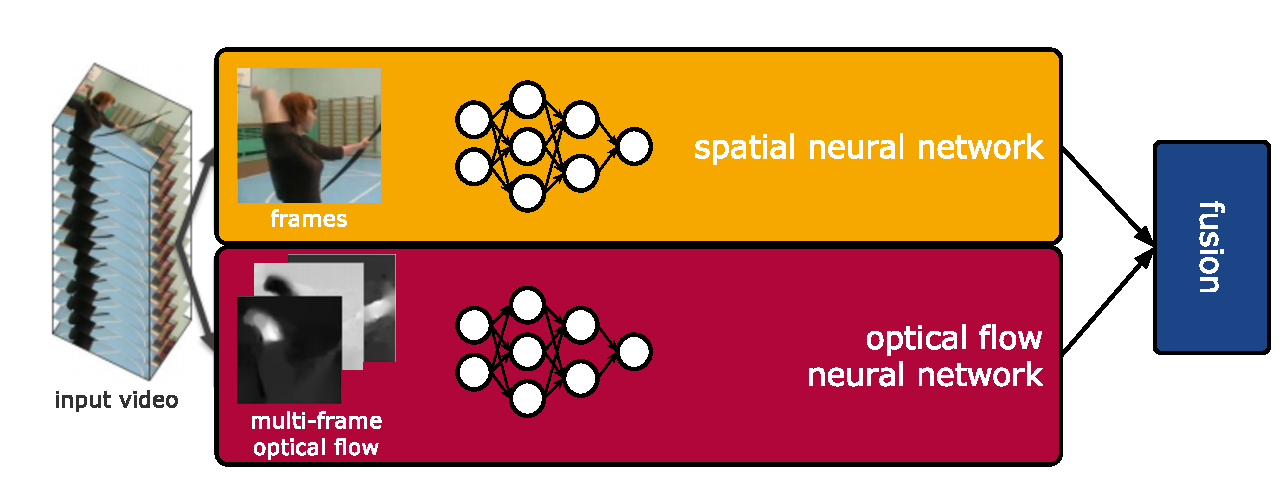
\includegraphics[scale=.7]{images/net_architecture.eps}
	\caption{Our neural network architecture consisting of three components: \emph{spatial}, \emph{flow} and \emph{fusion}. The \emph{spatial} and \emph{flow} neural network are convolutional neural networks. The predictions of both networks are combined in the third \emph{fusion} network.}
	\label{fig:architecture}
\end{figure}

During our research we tried out different neural networks, which will be presented in this section.
Additionally, we will summarize the results and hyperparameters, which were used for the training.

\subsection{Modifications to Caffe}

Working with a neural network consisting of LSTMs requires two different inputs:
On the one hand the raw pixel values and on the other hand a binary tagging sequence.
The tagging sequence tells the LSTM, where a new training example starts.
This is important, as there is more than one training sequence per batch.
A tagging sequence consist of 0's and 1's.
A 1 indicates the beginning of a new sequence.
For generating this tagging sequence we wrote a new data-generation strategy for the \emph{DummyData} layer.
This layer is meant to generate artificial data: Existing implementations generate constant values, uniformly distributed and Gaussian distributed data etc.

An example of the dummy data layer can be found in Listing~\ref{lst:seq-layer}.
The layer has the following two parameters:
The \texttt{shape} parameter defines the output shape of the tagging blob, i.e. \texttt{16 x 4} in the example.
The second parameter \texttt{data\_filler} sets the concrete parameters for the dummy data.
In our case, we specify the tagging sequence data generation type.
The parameter \texttt{value} specifies the length of a sequence.
In the example, this means that there is a single one, followed by 15 zeros.

\begin{lstlisting}[language=sh, caption=Sequence Layer, label=lst:seq-layer]
layer {
	name: "sequence"
	type: "DummyData"
	top: "sequence"
	dummy_data_param {
		shape {
			dim: 16
			dim: 4
		}
		data_filler {
			type: "sequence"
			value: 16
		}
	}
}
\end{lstlisting}

In order to create stacked optical flow data we made a second modification to Caffe.
As mentioned in section \ref{subsec:convert_imageset_multi}, we added a utility script to bundle a list of images into a database of stacked images.

\subsection{Experiment infrastructure}
For running experiments with different parameter settings, we build a script, which helps with keeping track of different experiments.
It can be found in the \texttt{nets/*} subfolders under the name \texttt{train.sh}.
It is started like \texttt{train.sh dropout0.7fps30}, where the parameter indicates the name of the experiment.
This automatically creates a folder \texttt{experiments/20150907-100235\_dropout0.7fps30}, where the first numbers indicate the date and time of the experiment.
Before starting the experiment in Caffe, the script automatically copies the net and solver definitions to this folder.
After the training has finished or has been aborted, it copies the logs and the latest snapshots to the same folder.
It also automatically parses the logs and creates charts, which plot the iteration number against training loss, learning rate and test accuracy.
We used this script for all of our experiments and think it is of great value.

\subsection{Spatial}
\label{subsec:spatial}
For our \emph{spatial} net we relied on finetuning two well-established networks from the University of Oxford.
CNN-M-2048 \cite{chatfield2014return} is medium sized net of 8 layers (5 convolutional, 3 fully-connected) trained in the ILSVRC-2012 data.
The complete layer architecture can be found in table \ref{table:cnn-m-208}.

\begin{table}[H]
\centering
\caption{CNN-M-2048 architecture}
\label{table:cnn-m-208}
\begin{tabularx}{\textwidth}{XXXXXXXX}
\toprule
conv1 & conv2 & conv3 & conv4 & conv5 & full6  & full7 & full8 \\ \midrule
96x7x7  stride 2, pad 0  LRN, x2 pool  &
256x5x5 stride 2, pad 1  LRN, x2 pool  &
512x3x3 stride 1, pad 1   &
512x3x3 stride 1, pad 1   &
512x3x3 stride 1, pad 1   &
4096  dropout  &
2048  dropout  &
1000  softmax  \\
\bottomrule
\end{tabularx}
\end{table}

Later we were able to evaluate the very deep 19 layer VGG-19 \cite{simonyan2014very} network\footnote{\url{https://gist.github.com/ksimonyan/3785162f95cd2d5fee77\#file-readme-md}}.

We experimented with different configurations of the learning rate, dropout rate, the number of finedtuned layers and with different amounts of input data. Some nets were trained with only 16 frames belonging to one video and others with all frames of the respective video. A complete overview can be seen in table \ref{table:spatial_results}.

\begin{table}[H]
\centering
\caption{Spatial Net Configurations}
\label{table:spatial_results}
\begin{tabularx}{\textwidth}{XXXXXXXXX}
\toprule
Net & Layers & Accuracy	& Learning Rate & Dropout Rate & Fine- tuned Layers	& Iterations	& FPS & LSTM Config \\ \midrule

CNN\_M & 8          & 67.90\% & 0.001 & 1 & 3 & 100,000 & 15 & \\
CNN\_M & 8          & 67.20\% & 0.001 & 1 & 3 &  31,000 & 15 & \\
CNN\_M & 8          & 68.30\% & 0.001 & 3 & 3 & 200,000 & 15 & \\
CNN\_M & 8          & 68.89\% & 0.001 & 5 & 3 & 134,000 & 15 & \\
CNN\_M & 8          & 06.19\% & 0.001 & 3 & 3 &   6,000 & 15 & \\
CNN\_M & 8          & 69.90\% & 0.001 & 7 & 3 &  76,000 & 15 & \\
CNN\_M & 7 + 2 lstm & 67.50\% & 0.001 & 7 & 3 & 180,000 & 15 & 1024 + 512 \\
CNN\_M & 7 + 2 lstm & 65.60\% & 0.001 & 7 & 3 &   7,000 & 15 & 256 + 256 \\
CNN\_M & 7 + 2 lstm & 65.80\% & 0.001 & 5 & 3 & 200,000 & 15 & 256 + 256 \\
CNN\_M & 7 + 1 lstm & 67.30\% & 0.001 & 5 & 2 &  85,000 & 15 & 256 \\
CNN\_M & 7 + 1 lstm & 66.60\% & 0.001 & 7 & 2 & 200,000 & 15 & 256 \\
CNN\_M & 7 + 1 lstm & 66.73\% &  0.01 & 7 & 2 & 200,000 & 15 & 256 \\
VGG19 & 19          & 73.40\% & 0.001 & 7 & 3 &       - & 15 & \\
VGG19 & 19          & 74.80\% & 0.001 & 7 & 4 &       - & 15 & \\
VGG19 & 19          & 74.10\% & 0.001 & 7 & 7 &       - & 15 & \\
VGG19 & 19          & 73.10\% & 0.001 & 7 & 3 &       - & 30 & \\
VGG19 & 19          & 75.30\% & 0.001 & 7 & 5 &       - & 30 & \\
VGG19 & 19          & 74.90\% & 0.001 & 7 & 6 &       - & 30 & \\
VGG19 & 19          & 74.60\% & 0.001 & 7 & 7 &       - & 30 & \\

\bottomrule
\end{tabularx}
\end{table}

As you can see from the different experiments, we achieved the best result using the CNN\_M net with 8 layers.
Having a learning rate of 0.001, a dropout rate of 7 and finetuning the last two layers results in an accuracy of 69.9\%.

\subsection{Flow}
\label{subsec:flow}
Due to the different nature of the flow data we could not rely on finetuning the same networks we used for the \emph{spatial} part, since these were trained on RGB images.
We tried using the CNN-M-2048 architecture for training from scratch but to no avail.
Our final approach is based a CNN-M-48 net trained on flow data by the University of Fudan \cite{wu2015modeling}.
However, due to differences in the optical flow data to ours we achieved rather poor results of only 44.3\% instead of the published 70\%.
Finetuning the network on our data yielded in better performance.
We applied the same testing configuration as described for the spatial part.
All results are listed in table \ref{table:flow_results}.

\begin{table}[H]
\centering
\caption{Flow Net Configurations}
\label{table:flow_results}
\begin{tabularx}{\textwidth}{XXXXXXXX}
\toprule
Net 		& Layers	& Accuracy	& Learning Rate 	& Dropout Rate	& Fine- tuned Layers	& Iterations	& Frames per Video \\ \midrule

CNN\_M & 8 & 55.50\%  & 0.001 & - & - &   2,500 & 16\\
CNN\_M & 8 & 58.99\%  & 0.001 & 7 & 3 &  22,000 & all \\
CNN\_M & 8 & 60.20\%  & 0.001 & 8 & 3 & 200,000 & all \\
CNN\_M & 8 & 13.37\%  & 0.01  & 8 & 3 &  90,000 & all \\
CNN\_M & 8 & 65.30\%  & 0.001 & 8 & 8 & 116,000 & all \\
CNN\_M & 8 & 63.10\%  & 0.001 & 5 & 8 &  75,000 & all \\
CNN\_M & 8 & 66.40\%  & 0.001 & 9 & 3 & 400,000 & all \\
CNN\_M & 8 & 62.50\%  & 0.001 & 9 & 4 & 130,000 & all \\
CNN\_M & 8 & 62.30\%  & 0.001 & 7 & 4 & 400,000 & all \\
CNN\_M & 8 & 59.80\%  & 0.001 & 9 & 4 &  20,000 & all \\
CNN\_M & 8 & 58.60\%  & 0.001 & 8 & 3 &  15,000 & all \\
CNN\_M & 8 & 59.10\%  & 0.001 & 9 & 3 & 150,000 & all \\

\bottomrule
\end{tabularx}
\end{table}

The best accuracy result for the \emph{flow} network is 66.4\%.
This was achieved by using a learning rate of 0.001, a dropout rate of 8 and finetuning the last 3 of the 8 layers.

\subsection{Fusion}
\label{subsec:fusion}

To combine the respective results from \emph{spatial} and \emph{flow} we need a third component.
For the \emph{fusion} part we can use an additional machine learning algorithm to further generalize our prediction results.
To establish a baseline, we applied a support vector machine (SVM) for the fusion.
We followed up by using neutral networks for the fusion.
In the following section we will present and evaluate different network configurations.

\subsubsection{Support Vector Machine}
To establish a baseline we applied a SVM to the respective \emph{spatial} and \emph{flow} output.
The feature vector from the \texttt{fc6}-layer from both CNNs, which results in 16 x 4096 features for 16 frames of one video each, was taken as an input to the SVM.
To combine the inputs of the CNNs, we used a \texttt{concat}-layer, which does not learn or change the input in any way.
For the SVM we used a solution offered by Caffe.
For this SVM equivalent in Caffe a single fully connected layer (with no other learnable parameters) is needed, directly followed by a hinge loss layer.
The number of outputs of the fully connected layer has to be chosen equal to the number of classes and provides the class predictions to the hinge loss layer.
The whole net can be seen in Figure~\ref{fig:svm_fusion}.
This approach resulted in a fusion accuracy of 75\%.

\begin{figure}[tb]
	\centering
	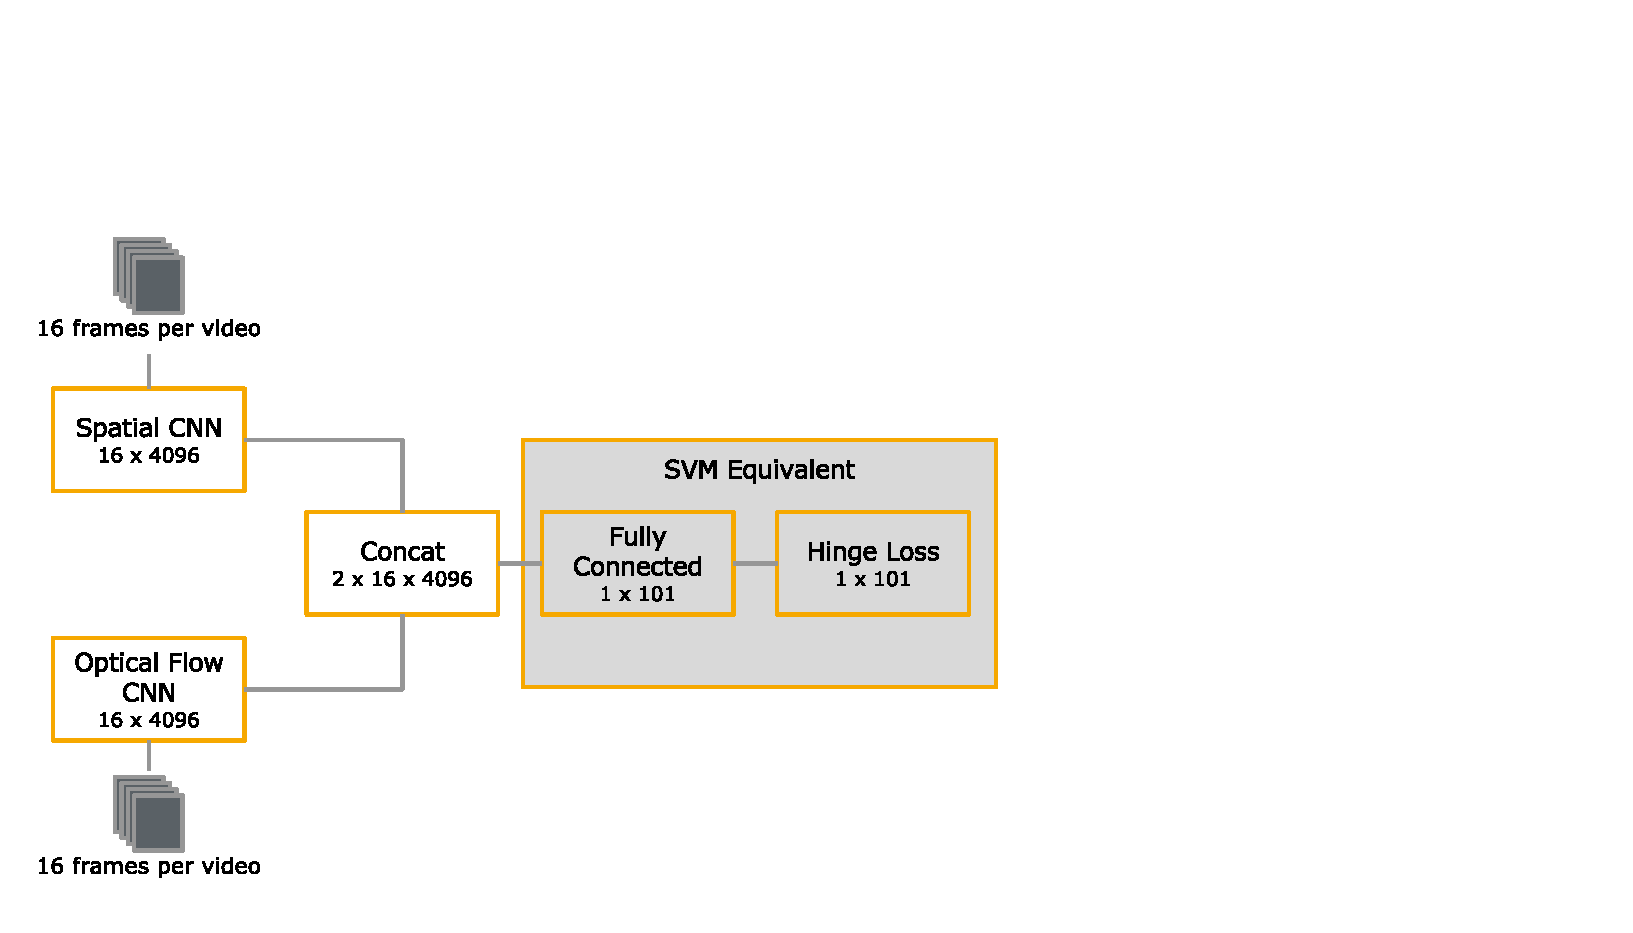
\includegraphics[scale=.7]{images/fusion_svm.eps}
	\caption{Fusion architecture using SVM: For the SVM a solution offered by Caffe consisting of a fully connected layer and a hinge loss layer was used.}
	\label{fig:svm_fusion}
\end{figure}

\subsubsection{Early Fusion}
Our \emph{early fusion} architecture was build on the fusion architecture presented by Wu et al.~\cite{wu2015modeling}.
We took the CNN\_Ms for \emph{spatial} and \emph{flow} presented above and build a fusion architecture on top of them.
We selected 16 frames per video as described in Section~\ref{sec:data} and pass them on to the CNNs for \emph{spatial} and \emph{flow}.
The CNNs were cut off after the \texttt{fc6}-layer resulting in an output of 1 x 4096 per frame.
Having 16 frames in total this corresponds to an input of 16 x 4096 for both \emph{spatial} and \emph{flow} for the fusion net.
The first step in the fusion network is to merge the 16 predictions of one video into one overall prediction for the whole video for both \emph{spatial} and \emph{flow}.
This is done by taking the average prediction.
A fully-connected layer is then trained with those predictions before we concatenate the predictions of \emph{spatial} and \emph{flow}.
Finally two fully-connected layers are trained on the merged predictions.
The output is defined by an accuracy layer.
The whole architecture is shown in Figure~\ref{fig:early_fusion}.

\begin{figure}[!htb]
	\centering
	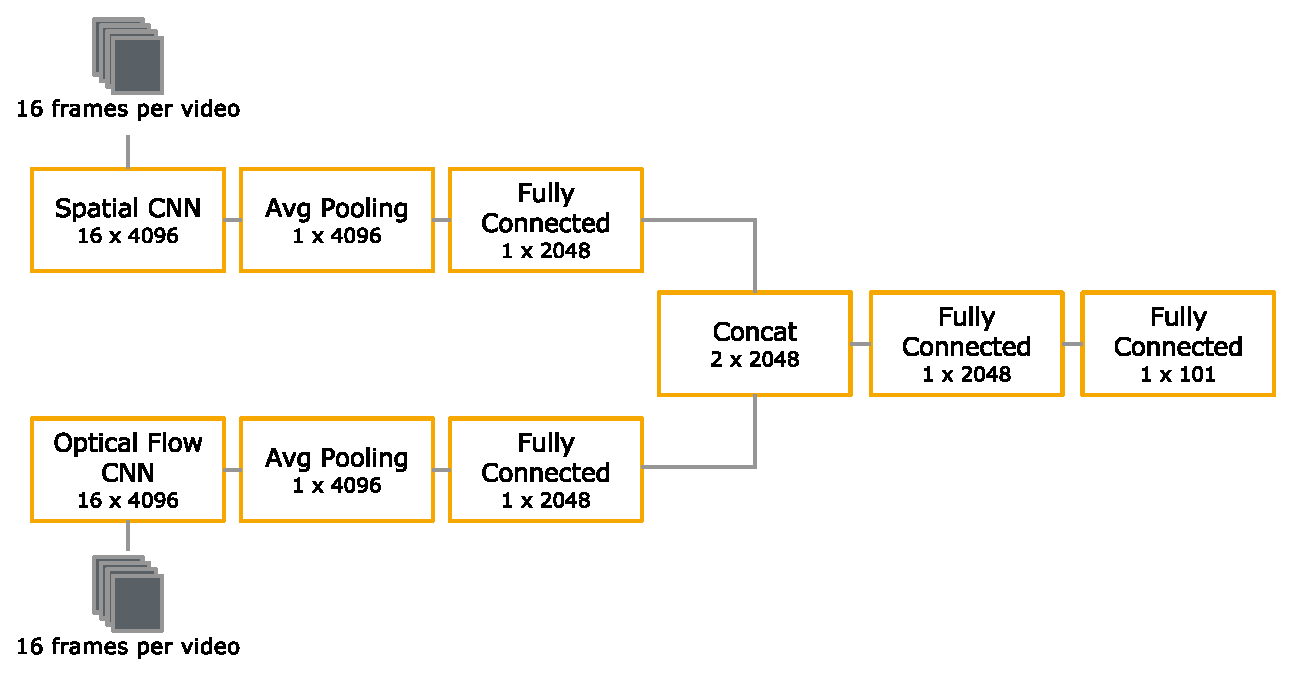
\includegraphics[scale=.7]{images/early_fusion.eps}
	\caption{Early fusion architecture: The predictions per frame of one video from the spatial and flow net are merged into one overall prediction per video each. Those predictions are then concatenated and trained via two fully connected layers.}
	\label{fig:early_fusion}
\end{figure}

\subsubsection{Middle Fusion}
In the \emph{middle} fusion the \texttt{fc6}-layer of the CNN for \emph{spatial} and \emph{flow} is changed so that the output is 1 x 101.
Having again 16 frames as input to the CNN the output and therefore input to the fusion is 16 x 101.
As in the \emph{early} fusion, the 16 prediction of one video are merged into one by taking the average prediction.
Afterwards, those predictions are trained via a fully connected layer and then concatenated.
In the end two fully connected layers are trained with the concatenated predictions.

\subsubsection{Late Fusion}
As in the \emph{middle} fusion the \texttt{fc6}-layer of the CNNs is adapted so that the output is 1 x 101.
Again 16 frames per video are used.
A fully connected layer is trained with the output of the CNNs, before the predictions are concatenated.
Afterwards, a fully connected layer is trained on those concatenated predictions, still leading to one prediction per frame (16 x 2048).
Now the 16 predictions per video are merged into one prediction by taking the average.
Finally, a fully connected layer is trained resulting in an output of 1 x 101.
The architecture of the \emph{late} fusion is shown in Figure~\ref{fig:late_fusion}.

\begin{figure}[!htb]
	\centering
	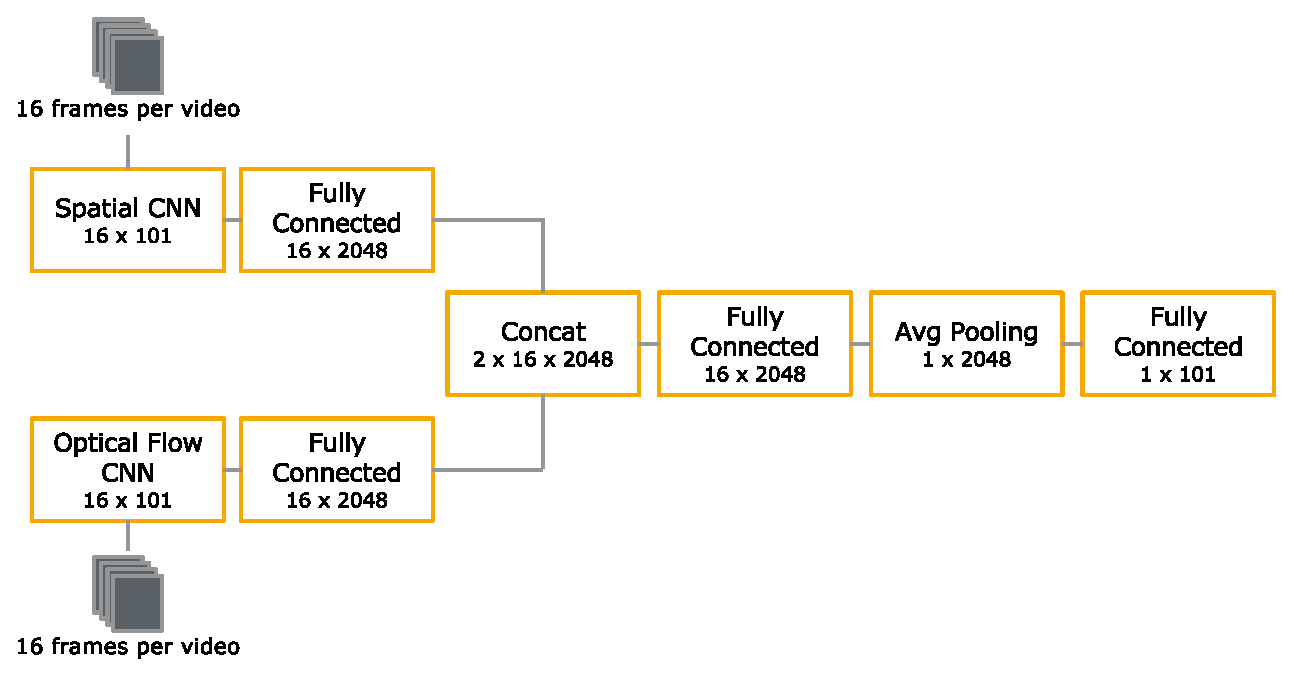
\includegraphics[scale=.7]{images/late_fusion.eps}
	\caption{Late fusion architecture: The predictions of the spatial and flow net are first concatenated before they are merged into one prediction.}
	\label{fig:late_fusion}
\end{figure}

\subsubsection{Experiments}

We tested the different fusion architectures with several parameters.
The results are listed in Table~\ref{table:fusion_results}.
For the CNNs we used those CNNs of \emph{spatial} and \emph{flow}, which lead to the best results.

\begin{table}[H]
\centering
\caption{Fusion Net Configurations}
\label{table:fusion_results}
\begin{tabularx}{\textwidth}{XXXXXXXX}
\toprule
Archi- tecture 		&  Accuracy	& Learning Rate 	& Dropout Rate	& Fusion Layers	& FPS & Batch Size \\ \midrule
Early  & 83.60\%  & 0.01  & 5 & 2 & 15 & 16 \\
Early  & 77.80\%  & 0.001 & 5 & 3 & 15 & 16 \\
Early  & 77.40\%  & 0.01  & 5 & 2 & 15 & 32 \\
Early  & 83.00\%  & 0.001 & 5 & 2 & 15 & 48 \\
Middle & 81.60\%  & 0.001 & 5 & 2 & 15 & 16 \\
Late   & 23.00\%  & 0.001 & 5 & 2 & 15 & 16 \\
SVM    & 74.90\%  & 0.001 & 5 & - & 15 & 16 \\
\bottomrule
\end{tabularx}
\end{table}
\todo[inline]{Fusion Experimente eintragen!}

As you can see our best overall result is 83.6\%.
This was achieved by using the the early fusion of the best VGG19 spatial network and the best CNN\_M temporal model.